\chapter{Introduction}
\label{ch:Introduction}

\stress{\textbf{Disclaimer to this document:} 
This is a template with some additional thesis information and a sample structure. 
The structure includes the chapters most commonly needed in a thesis. 
Neither the order nor the chapter titles are fixed and will most likely 
have to be adapted to your specific thesis. 
However, the notes here should help you to get an idea what each chapter 
could be about and how to use this template. 
When in doubt, please talk to your supervisor(s).}

Your thesis should start with an introduction. The introduction is supposed to motivate your thesis.
Discuss the relevance of your topic, why are you looking into it, why is it relevant in the field? Cite important research related to your motivation.
Briefly state the problem as in the abstract and repeat the contribution, for example in the form of research questions. 

Give an outline of your thesis.

Testing the glossaries package \gls{rmse}


Below, you will find an example figure (\Cref{fig:example}). Please use the caption of your figures to describe everything in the figure, additionally to what you have written about the figure in the text. Everyone should be able to understand the figure just reading its caption.

\begin{figure}[h!]%
\centering
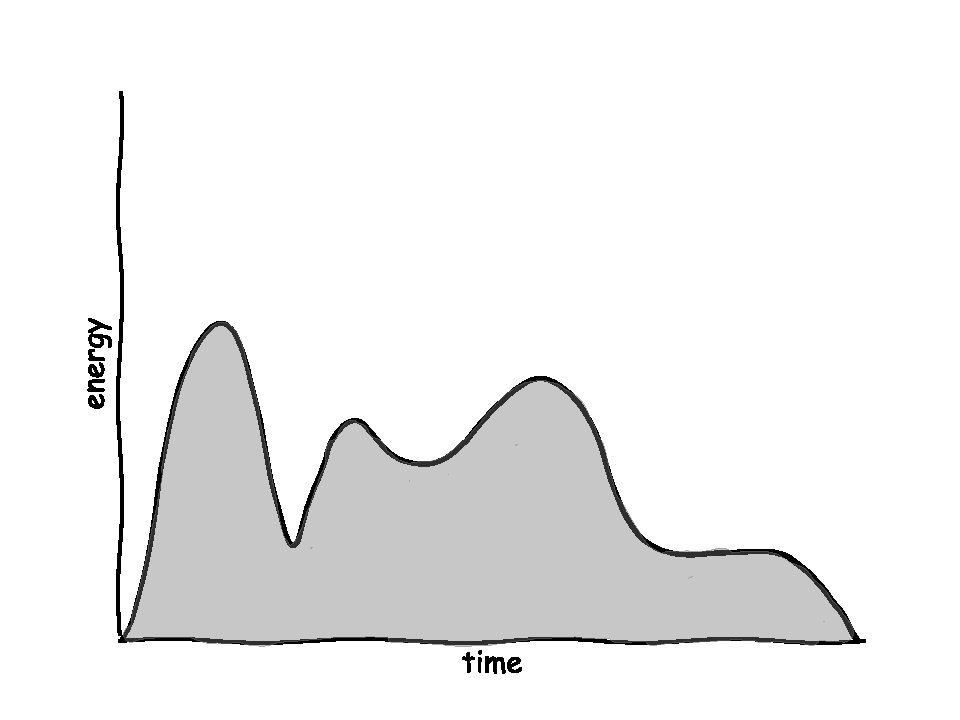
\includegraphics[width=0.5\columnwidth]{plots/Figure_2_demand}%
\caption{This is an example figure. It shows a fictional demand of energy (in grey) over time.}%
\label{fig:example}%
\end{figure}

\section{Motivation}
\label{sec:motivation}

% paragraph 1: 
% why is energy forecasting important (with citations)
% highlight solar forecasting as being of particular interest & 1-2 challenges

In the last decade, climate change has become an increasingly urgent problem. 
In order to reduce the amount of CO2 emitted due to energy production, 
the transition towards renewable energy sources is important. 
The photovoltaic share in the energy mix has seen continuous growth in 
the past years (\citeauthor{Snapshot2016}, \citedate{Snapshot2016}). 

Solar energy production fluctuates strongly as variables such as the weather change. 
\Textcite{Meer2018} argue that accurate forecasting of power generation is needed to properly 
integrate the renewable energy sources into the energy generation mix. 
In terms of forecasting methods, solar power is 
an interesting problem since it can be modeled through predictor variables 
like surface solar radiation, total cloud cover and precipitation 
for which high-quality forecasts from numerical weather prediction models are readily available. 

% paragraph 2: 
% motivate the importance of probabilistic solar forecasting
% solar forecasting is immature in comparison to other types

Energy forecasting has traditionally focused on point forecasts 
but nowadays, there is a substantial interest in probabilistic forecasts.
Because modeling the uncertainty of a forecast is relevant for planning the energy household of the electric grid, 
probabilistic forecasts make sense instead of only point forecasts (\citeauthor{Meer2018}, \citedate{Meer2018}). 
One challenge is to find the most effective method from all different probabilistic forecasting methodologies. 
\Textcite{Hong2016} state that wind power forecasting is 
more mature than solar energy forecasting.
This is most likely due to 
wind power forecasting being the closest to meteorological forecasting, 
where probabilistic forecasting is well-established and commonly accepted. 

% paragraph 3: 
% motivate deep learning for probabilistic solar forecasting
% motivate nonparametric deep learning for probabilistic solar forecasting
% highlight how there is no comparison yet

Because of the large amount of data that is being used for solar power forecasting, it makes sense to look at 
deep learning models for probabilistic solar forecasting. 
Deep learning often provides good results for complex problems with a lot of data to process. 
Generally, probabilistic forecasts can be distinguished into two types of forecasts: parametric, and nonparametric ones. 
Parametric learning assumes an underlying probability distribution, e.g., \(\mathcal{N}(\mu, \sigma^2)\). Here, the parameters 
of the distribution are estimated. 
Nonparametric learning does not make these assumptions. 
The advantage here is that this type of learning is applicable to problems where the underlying 
probability distribution class is unknown or difficult to specify -- like in solar energy forecasting. 

% paragraph 4:
% explain what you do in this thesis
% introduce models compared
% introduce data set

For this reason, we compare three different nonparametric machine learning models 
that tackle the probabilistic solar energy forecasting problem. 
The three models we take a look at are 
\begin{enumerate}
    \item Quantile Regression Forests (QRF) proposed by \Textcite{Meinshausen2006},
    \item Nearest Neighbor Quantile Filters (NNQF) proposed by \Textcite{Ordiano2019} and
    \item Spline Quantile Functions Recurrent Neural Network (SQF-RNN) proposed by \Textcite{Gasthaus2019}.
\end{enumerate}
All of these models are so called distributional regression methods, meaning 
they predict a probability distribution and try to minimize a loss function 
given the distribution and the target data.
We evaluate the models on the Global Energy Forecasting Competition 2014 (GEFCom2014) dataset and compare how well they perform 
in different metrics like the pinball loss (cf. \ref{sec:pinball-loss-explanation}), the energy score and PIT histograms. 

\section{Related Work}
\label{sec:related-work}

This section covers related work concerning solar energy forecasting as well as 
the different models that we look at. 
\Textcite{Hong2016} discusses the importance of solar energy, wind energy, electric load 
and electric price forecasting. They summarize the recent research progress on probabilistic 
energy forecasting and introduce the Global Energy Forecasting Competition 2014 (GEFCom2014).
\Textcite{Meinshausen2006} proposes the Quantile Random Forests method. He describes 
how it works, gives numerical examples that undermine its predictive performance
and provides proofs for some of the model's properties like consistency. 
\Textcite{Ordiano2019} introduce the Nearest Neighbors Quantile Filters (NNQF) method. 
They explain the advantages and test the model's performance on the GEFCom2014 dataset. 
We will also try out the model on the GEFCom2014 dataset and evaluate 
it in multiple kinds of manners.
\Textcite{Salinas2017} introduce the DeepAR model -- a model for probabilistic forecasting 
with autoregressive recurrent neural networks. They evaluate the model on several 
real-world data sets and show that this model has accuracy improvements of around 
\(15\%\) compared to other state-of-the-art methods.
\Textcite{Gasthaus2019} propose the SQF-RNN model, an extension of the DeepAR model 
that is supposed to be a more flexible method for probabilistic forecasting 
by modeling the quantile function with splines instead of a fixed distribution class.
They empirically demonstrate its effectiveness by evaluating the model on several real-world 
data sets and comparing it with the DeepAR model.

In this thesis, we will be comparing these models and discussing 
their suitability for solar power generation.

\section{Problem description}
\label{sec:problem-description}

This thesis tries to answer the following research questions:
\begin{enumerate}
    \item How do nonparametric models perform in comparison to parametric models 
    on the probabilistic solar power generation forecasting problem?
    \item How do the models perform based on various aspects of forecast 
    quality? Are the forecasts sharp and calibrated? How large are the variances and losses?
    \item Are there challenges and advantages of the chosen GEFCom2014 setting?
\end{enumerate}